\paragraph{Anchoring the simulator.} The decoder-quality dial is anchored to two real reference points:
\begin{itemize}
\item A Wiener filter with FALCON's 600\,ms history, trained on all held-in days, reaches R$^2$=\RealRsqMulti{} on real minival data. The nominal level is the dial setting whose simulated R$^2$ is closest to this value: \NominalRsq{} at $\kappa=\NominalKappa$.
\item The closed-loop decoder itself (10 taps, one session) reaches only \RealRsq{} on real data, at the low end of the dial.
\end{itemize}
Results at the nominal level use \Episodes{} paired episodes per method and scenario.

\begin{table*}[t]
\centering\small
\adjustbox{max width=\textwidth}{\begin{tabular}{l ccccc ccc cc}
\toprule
& \multicolumn{5}{c}{Standard (3 objects)} & \multicolumn{3}{c}{Change of mind} & \multicolumn{2}{c}{Clutter (5 obj.)} \\
\cmidrule(lr){2-6}\cmidrule(lr){7-9}\cmidrule(lr){10-11}
Method & Succ. & Wrong & Time (s) & Path eff. & User share & Succ. & Wrong & Yield (s) & Succ. & Wrong \\
\midrule
Decoder only & 0.02 & 0.00 & 19.0 & 0.17 & 1.00 & 0.05 & 0.00 & 3.24 & 0.05 & 0.00 \\
Fixed blend & 0.88 & 0.02 & 6.9 & 0.69 & 0.29 & 0.88 & 0.07 & 2.66 & 0.75 & 0.02 \\
Distance blend [Downey'16] & 1.00 & 0.00 & 8.3 & 0.51 & 0.76 & 0.47 & 0.45 & 3.00 & 0.93 & 0.07 \\
Confidence blend [Dragan'13] & 0.90 & 0.00 & 7.2 & 0.66 & 0.24 & 0.92 & 0.07 & 2.26 & 0.78 & 0.02 \\
Hindsight assist [Javdani'15] & 0.90 & 0.02 & 6.8 & 0.67 & 0.49 & 0.68 & 0.23 & 2.61 & 0.70 & 0.02 \\
\textbf{DASA (ours)} & 1.00 & 0.00 & 5.2 & 0.83 & 0.29 & 1.00 & 0.00 & 0.73 & 1.00 & 0.00 \\
\bottomrule
\end{tabular}
}
\caption{Simulated closed loop at the nominal decoder quality (offline R$^2$=\NominalRsq). \emph{Wrong}: closed the gripper on a non-goal object. \emph{Time} and \emph{path efficiency} are over successful episodes. \emph{User share}: the user's share of the command norm. \emph{Yield}: median time from the change of mind until the goal estimate settles on the new goal. Hyper-parameters of every method were tuned on separate seeds.}
\label{tab:sa}
\end{table*}

\begin{figure*}[t]
\centering
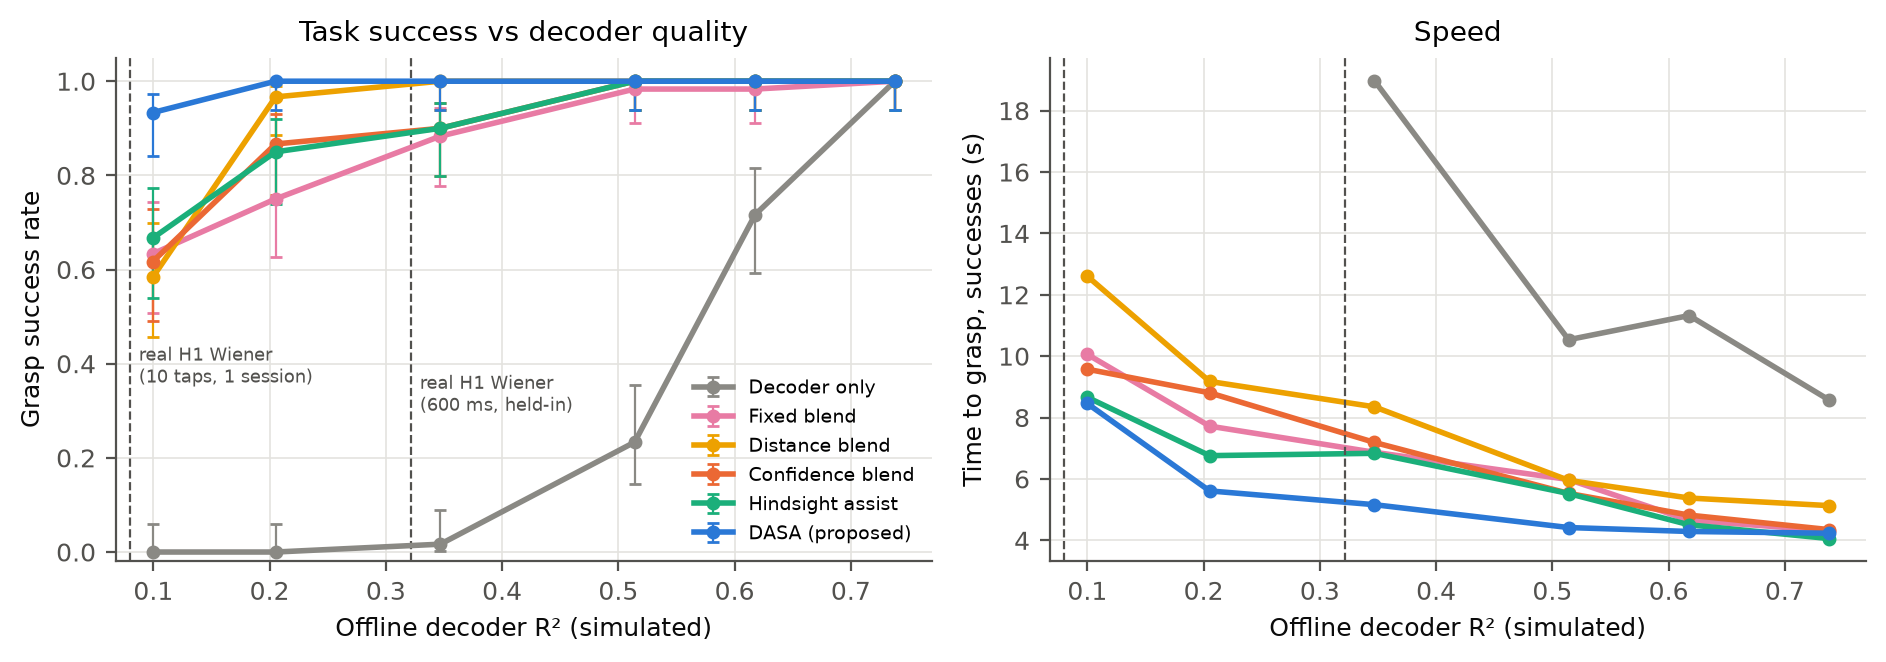
\includegraphics[width=0.85\textwidth]{figures/success_vs_r2.png}
\caption{Success and time-to-grasp against simulated offline decoder R$^2$ (Wilson 95\% CIs; 60 episodes per point). Dashed lines mark two real-data references: the closed-loop decoder configuration on its own session, and a FALCON-style Wiener filter on held-in data.}
\label{fig:sweep}
\end{figure*}

\paragraph{Assistance is necessary at today's decoding accuracy.}
\begin{itemize}
\item \textbf{Decoder only.} Without assistance the simulated user grasps the goal in \SuccDirect{} of standard episodes at the nominal level (Table~\ref{tab:sa}). The arm still reaches the vicinity of the goal; what fails is the final 3\,cm/20$^\circ$ alignment and a clean gripper closure. Decoder-only success needs offline R$^2\gtrsim0.6$ to exceed 50\% (Fig.~\ref{fig:sweep}).
\item \textbf{Every assisted method} raises success to 0.88--1.00 at the nominal level. This matches the clinical observation that shared control rescues grasping~\cite{downey2016blending}.
\end{itemize}

\paragraph{DASA is faster, straighter and never grasps the wrong object.}
On the standard task:
\begin{itemize}
\item DASA succeeds in \SuccDASA{} of episodes and grasps in \TimeDASA\,s on average, versus \TimeConfidence\,s for confidence blending and \TimeHindsight\,s for hindsight assistance.
\item Its path efficiency is the highest of all methods.
\item Its paired success advantage is significant over fixed blending (McNemar $p$=\PStdFixed), confidence blending ($p$=\PStdConfidence) and hindsight assistance ($p$=\PStdHindsight).
\item Distance blending also reaches \SuccDistance{}, but is slower (\TimeDistance\,s), because assistance only switches on inside the grasp envelope.
\end{itemize}
DASA's goal estimate is correct earlier in the episode than any baseline's (Fig.~\ref{fig:goal}). The reason: its likelihood uses all seven decoded dimensions, wrist and grasp included, and it weights them by their measured reliability.

\paragraph{Clutter.} With five objects at least 8\,cm apart:
\begin{itemize}
\item MaxEnt-based methods drop to \ClutSuccConfidence{} (confidence blending) and \ClutSuccHindsight{} (hindsight).
\item Distance blending holds up at \ClutSuccDistance{}, but grasps the wrong object in \ClutWrongDistance{} of episodes.
\item DASA keeps \ClutSuccDASA{} success with no wrong grasps.
\end{itemize}

\begin{figure}[t]
\centering
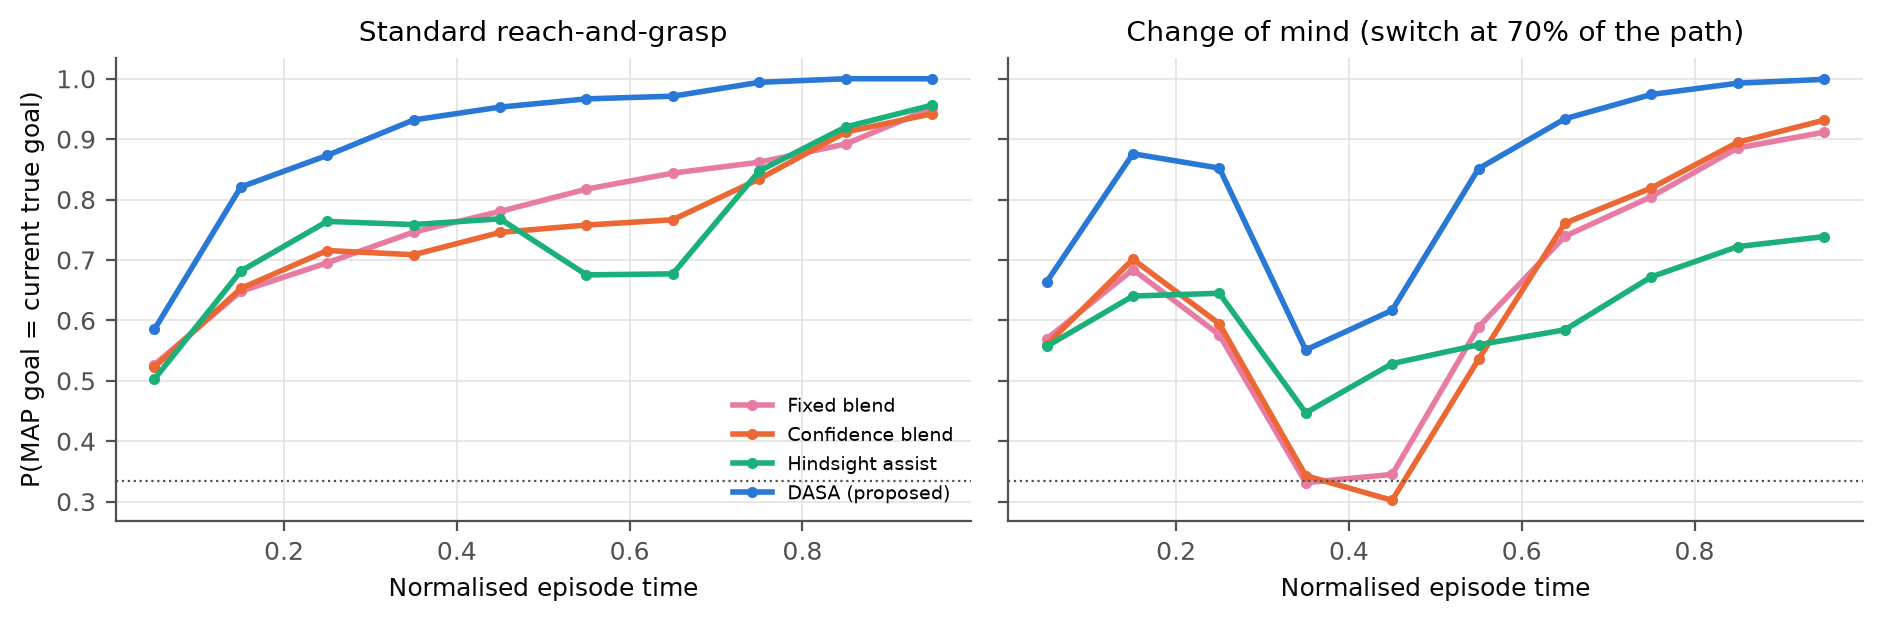
\includegraphics[width=\columnwidth]{figures/goal_inference.png}
\caption{Probability that the MAP goal equals the user's current goal over normalised episode time (nominal decoder). Dotted line: chance with three objects.}
\label{fig:goal}
\end{figure}

\paragraph{Changing one's mind: assistance must yield.}
In this scenario the user switches goals after covering 70\% of the way to the first object, by which point every method's assistance is committed.
\begin{itemize}
\item \textbf{Distance blending} is the worst. It assists toward whichever object is nearest, so it grasps the abandoned object in \ComWrongDistance{} of episodes.
\item \textbf{Hindsight assistance} also grasps the wrong object in \ComWrongHindsight{} of episodes. Its accumulated posterior keeps pulling the arm toward the first goal.
\item \textbf{DASA} settles on the new goal after a median of \YieldDASA\,s, versus \YieldConfidence\,s for confidence blending and \YieldHindsight\,s for hindsight. It succeeds in \ComSuccDASA{} of change-of-mind episodes with no wrong grasps (Fig.~\ref{fig:com}).
\end{itemize}
The ablations (below) show that the switching prior and the calibrated likelihood are what make this fast yielding possible.

\begin{figure*}[t]
\centering
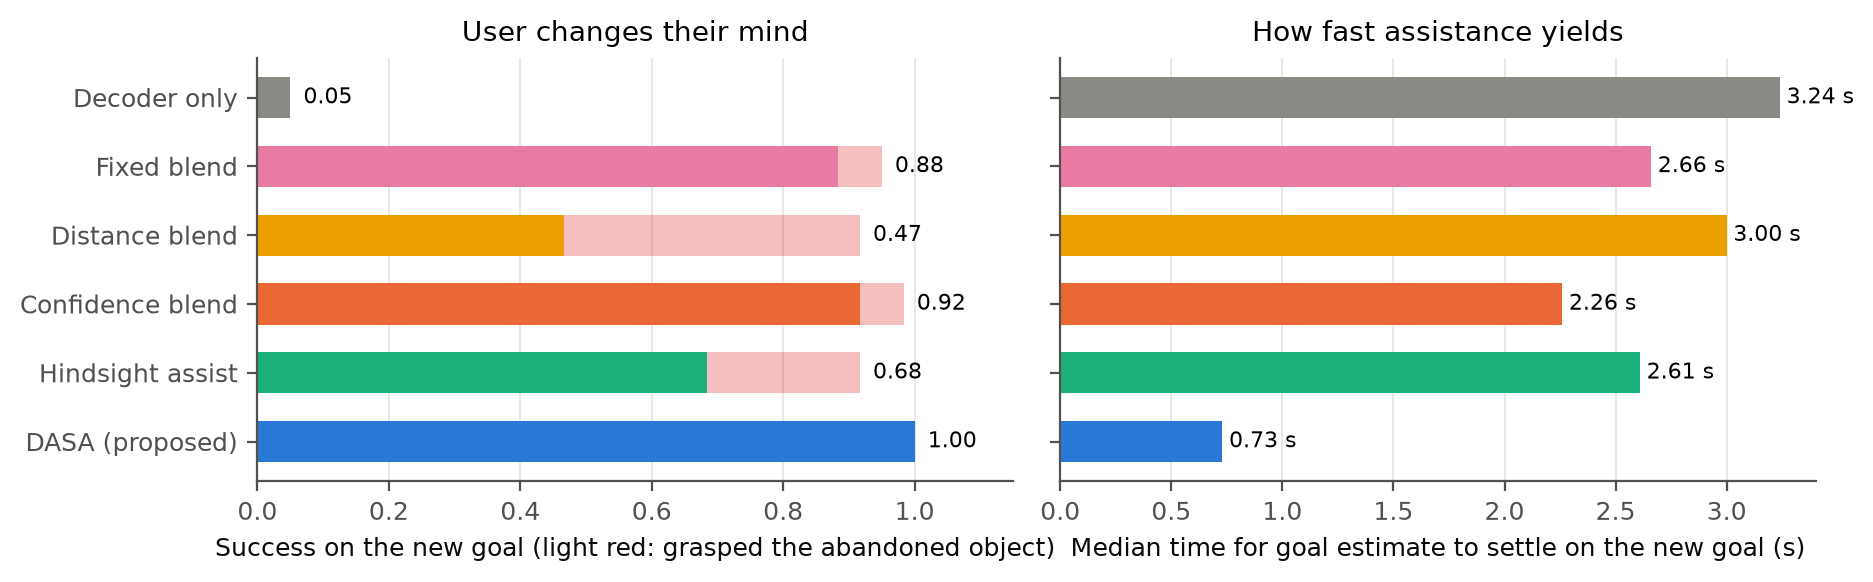
\includegraphics[width=0.85\textwidth]{figures/change_of_mind.png}
\caption{Change-of-mind scenario at the nominal decoder. Left: success on the new goal; shaded red marks episodes that closed on the abandoned object. Right: median yield latency.}
\label{fig:com}
\end{figure*}

\paragraph{Authority versus performance.}
Success can always be bought by taking control away from the user, so we sweep each method's assistance strength (Fig.~\ref{fig:authority}).
\begin{itemize}
\item At a user share of about 0.5, DASA ($\alpha_{\max}=0.6$) is still at ceiling success. Confidence and fixed blending at a similar share succeed in only 0.57--0.64 of episodes.
\item Hindsight assistance, which by construction keeps the user's command and adds a correction, sits near a 0.5 share at 0.80--0.83 success.
\end{itemize}
DASA therefore offers a strictly better frontier in this simulation: it can return half of the control to the user without losing success. This matters because users value authority~\cite{javdani2015shared,gopinath2017human}.

\begin{figure*}[t]
\centering
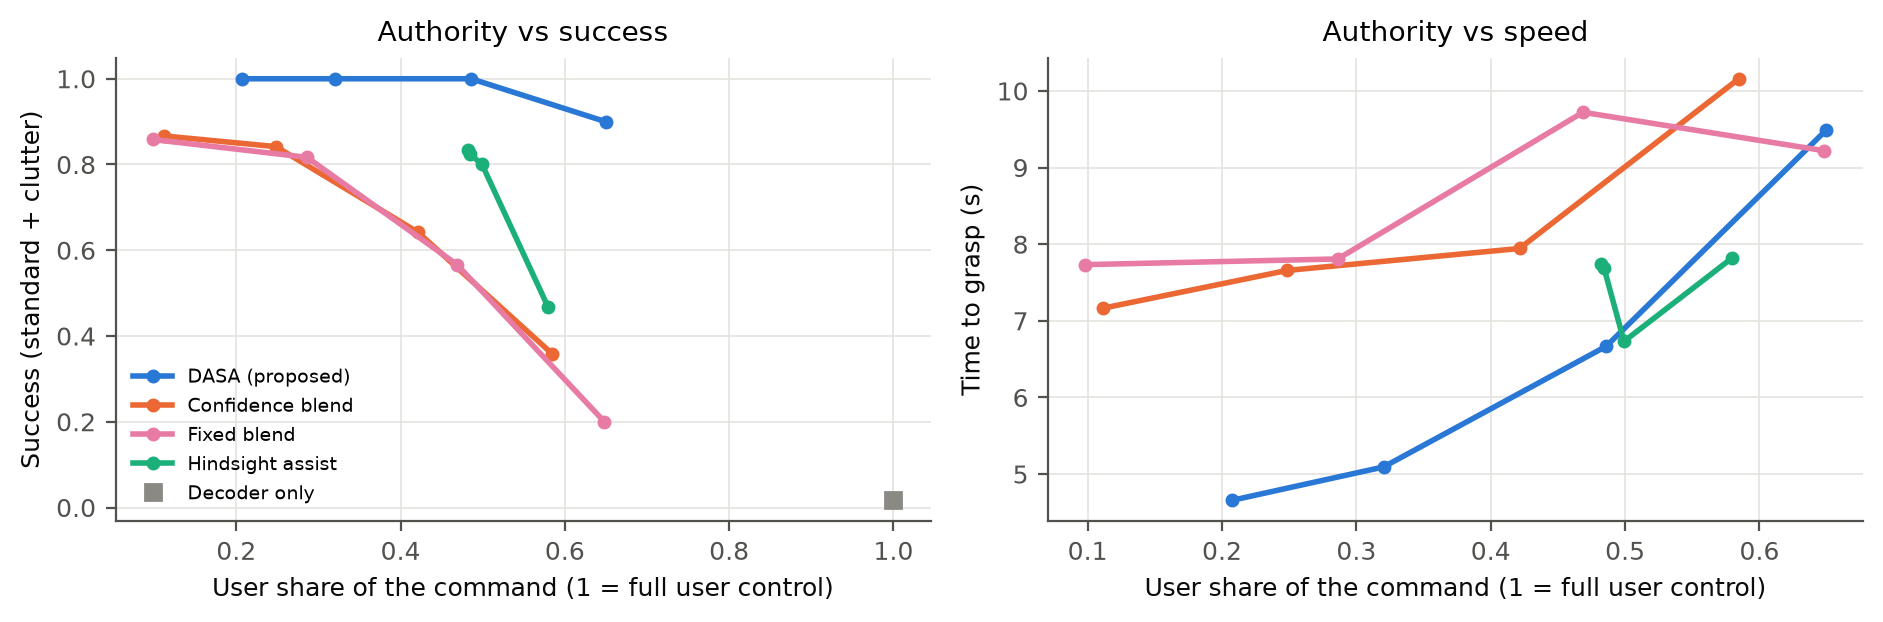
\includegraphics[width=0.85\textwidth]{figures/authority_tradeoff.png}
\caption{Authority--performance trade-off at the nominal decoder (standard + clutter episodes). Each method's assistance strength is swept: $\alpha_{\max}$ for DASA and confidence blending, $\alpha$ for fixed blending, $\lambda$ for hindsight assistance. Upper right is better.}
\label{fig:authority}
\end{figure*}

\paragraph{Ablations.} Table~\ref{tab:abl} and Fig.~\ref{fig:abl} report the ablations at the nominal level and at the weakest decoder (R$^2\approx0.1$). At the nominal level DASA saturates, so most differences there appear as slower yielding rather than as lost successes.
\begin{itemize}
\item \textbf{Autocorrelation correction} is the most important component. Without it the posterior becomes over-confident on correlated decoder errors. At the weakest decoder, success falls from 0.93/0.85/0.87 (standard / change of mind / clutter) to 0.70/0.47/0.27. At the nominal level, yielding slows from 0.73\,s to 3.6\,s.
\item \textbf{The calibrated error model} ($G$, $\Sigma$, $\tau$ replaced by identity) is the next most important. At the weakest decoder, success falls to 0.77/0.63/0.68, and nominal yielding slows to 4.1\,s.
\item \textbf{The switching prior} matters for changes of mind. Without it, nominal yielding takes 2.5\,s; at the weakest decoder, change-of-mind success drops to 0.75 and wrong grasps double (0.20 vs 0.10).
\item \textbf{The consistency gate} has no effect at the nominal level. At the weakest decoder it raises change-of-mind success from 0.73 to 0.85, at a negligible cost on the standard task.
\item \textbf{A user model with the wrong speed} (assumed 2$\times$ slower) costs little at the nominal level. At the weakest decoder, clutter success drops to 0.63.
\item \textbf{A switching prior on MaxEnt inference does not work}, even with its temperature re-tuned: success is 0.30 or lower. A MaxEnt likelihood is too weak and too poorly calibrated to overcome the switching hazard, so the posterior never concentrates. The switching prior is usable only with a likelihood calibrated to the decoder's noise.
\end{itemize}

\begin{table}[t]
\centering\scriptsize
\setlength{\tabcolsep}{3pt}
\adjustbox{max width=\columnwidth}{\begin{tabular}{l ccc ccc}
\toprule
& \multicolumn{3}{c}{Nominal (R$^2$ 0.35)} & \multicolumn{3}{c}{Weakest (R$^2$ 0.10)} \\
\cmidrule(lr){2-4}\cmidrule(lr){5-7}
Variant & Std. & Change & Clutter & Std. & Change & Clutter \\
\midrule
DASA (full) & 1.00 & 1.00 & 1.00 & 0.93 & 0.85 & 0.87 \\
$-$ consistency gate & 1.00 & 1.00 & 1.00 & 0.95 & 0.73 & 0.87 \\
$-$ switching prior & 1.00 & 0.97 & 1.00 & 0.93 & 0.75 & 0.88 \\
$-$ autocorrelation correction ($\tau{=}1$) & 1.00 & 0.98 & 0.97 & 0.70 & 0.47 & 0.27 \\
$-$ calibrated error model ($G{=}I,\Sigma{=}I,\tau{=}1$) & 1.00 & 1.00 & 1.00 & 0.77 & 0.63 & 0.68 \\
mismatched user model (speed $\times0.5$) & 1.00 & 0.98 & 1.00 & 0.83 & 0.80 & 0.63 \\
Confidence blend + switching prior & 0.10 & 0.03 & 0.07 & 0.00 & 0.02 & 0.02 \\
Confidence + switching, $\beta$ re-tuned & 0.30 & 0.35 & 0.20 & 0.02 & 0.02 & 0.00 \\
\bottomrule
\end{tabular}
}
\caption{Ablations: success rate (60 episodes per cell) at the nominal and the weakest simulated decoder.}
\label{tab:abl}
\end{table}

\begin{figure*}[t]
\centering
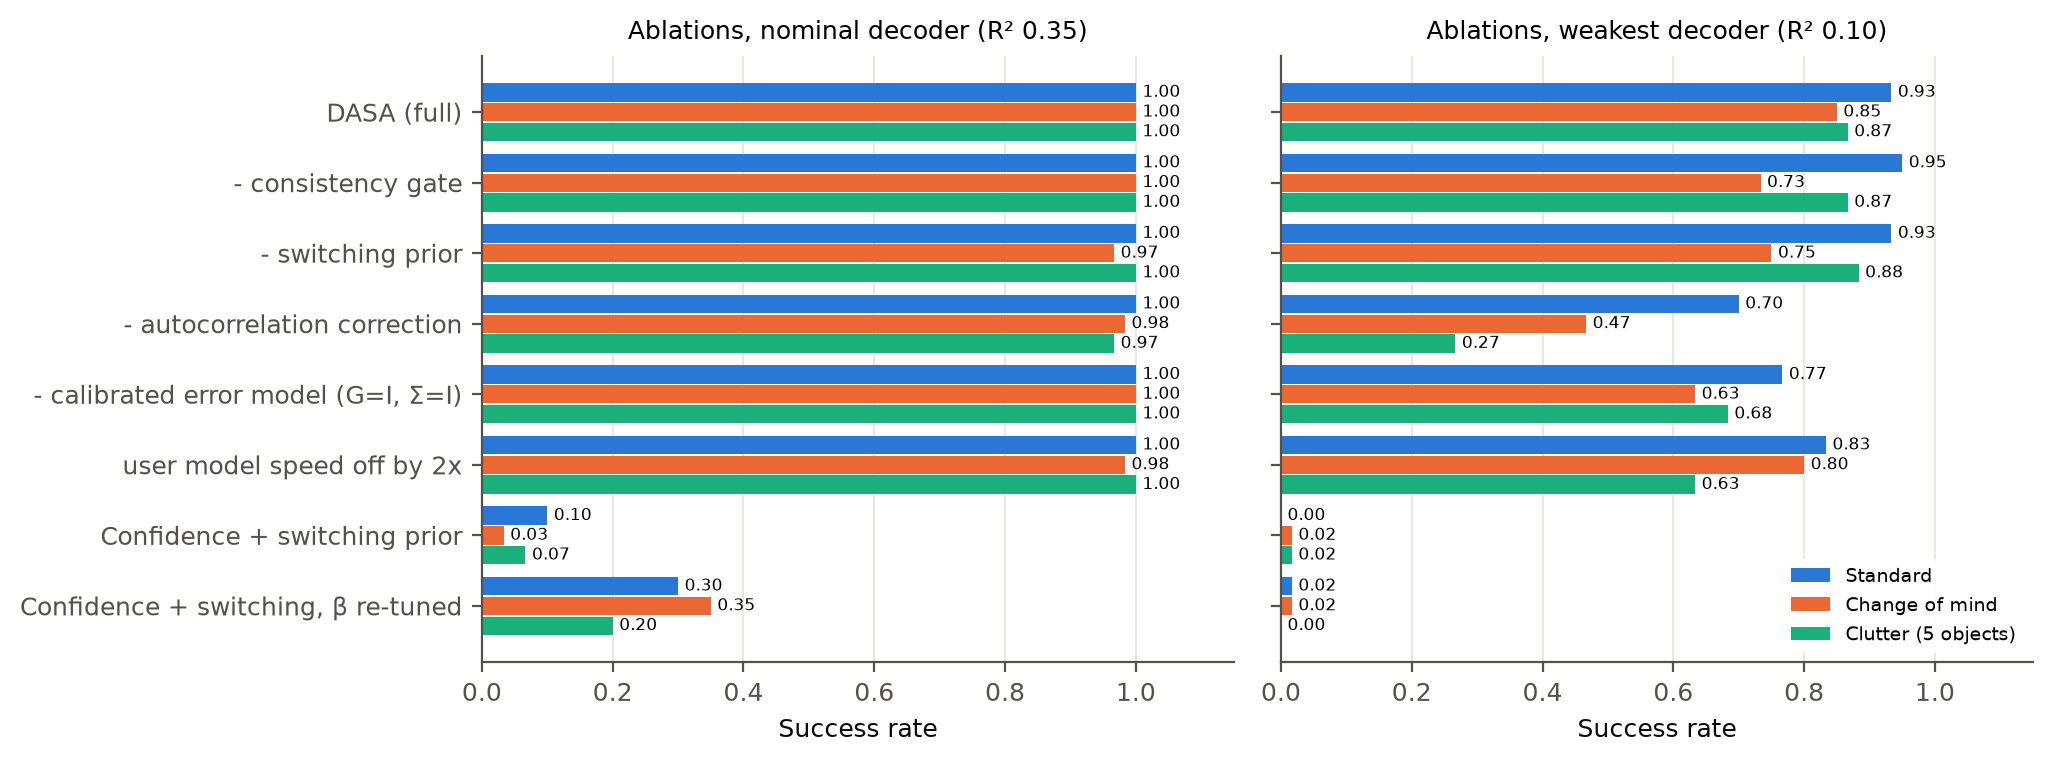
\includegraphics[width=0.9\textwidth]{figures/ablations.png}
\caption{Ablations of DASA, and MaxEnt inference with a switching prior.}
\label{fig:abl}
\end{figure*}

\paragraph{Safety filter.} The same safety filter is applied after every method.
\begin{itemize}
\item With assistance the speed cap rarely engages: about 0.1 times per episode for DASA at the nominal level, against about 15 per episode for the noisy decoder alone.
\item Across all \SafetyEpisodes{} simulated episodes of the run, the link--table check never had to block a motion (\SafetyLinkTable{} episodes). Joint-limit clipping occurred in \SafetyJointLimit{} episodes, workspace clipping in \SafetyWorkspace{}, and table-plane clipping in \SafetyTablePlane{} (mostly under decoder-only control).
\end{itemize}
Example trajectories are shown in Fig.~\ref{fig:episodes}.

\begin{figure*}[t]
\centering
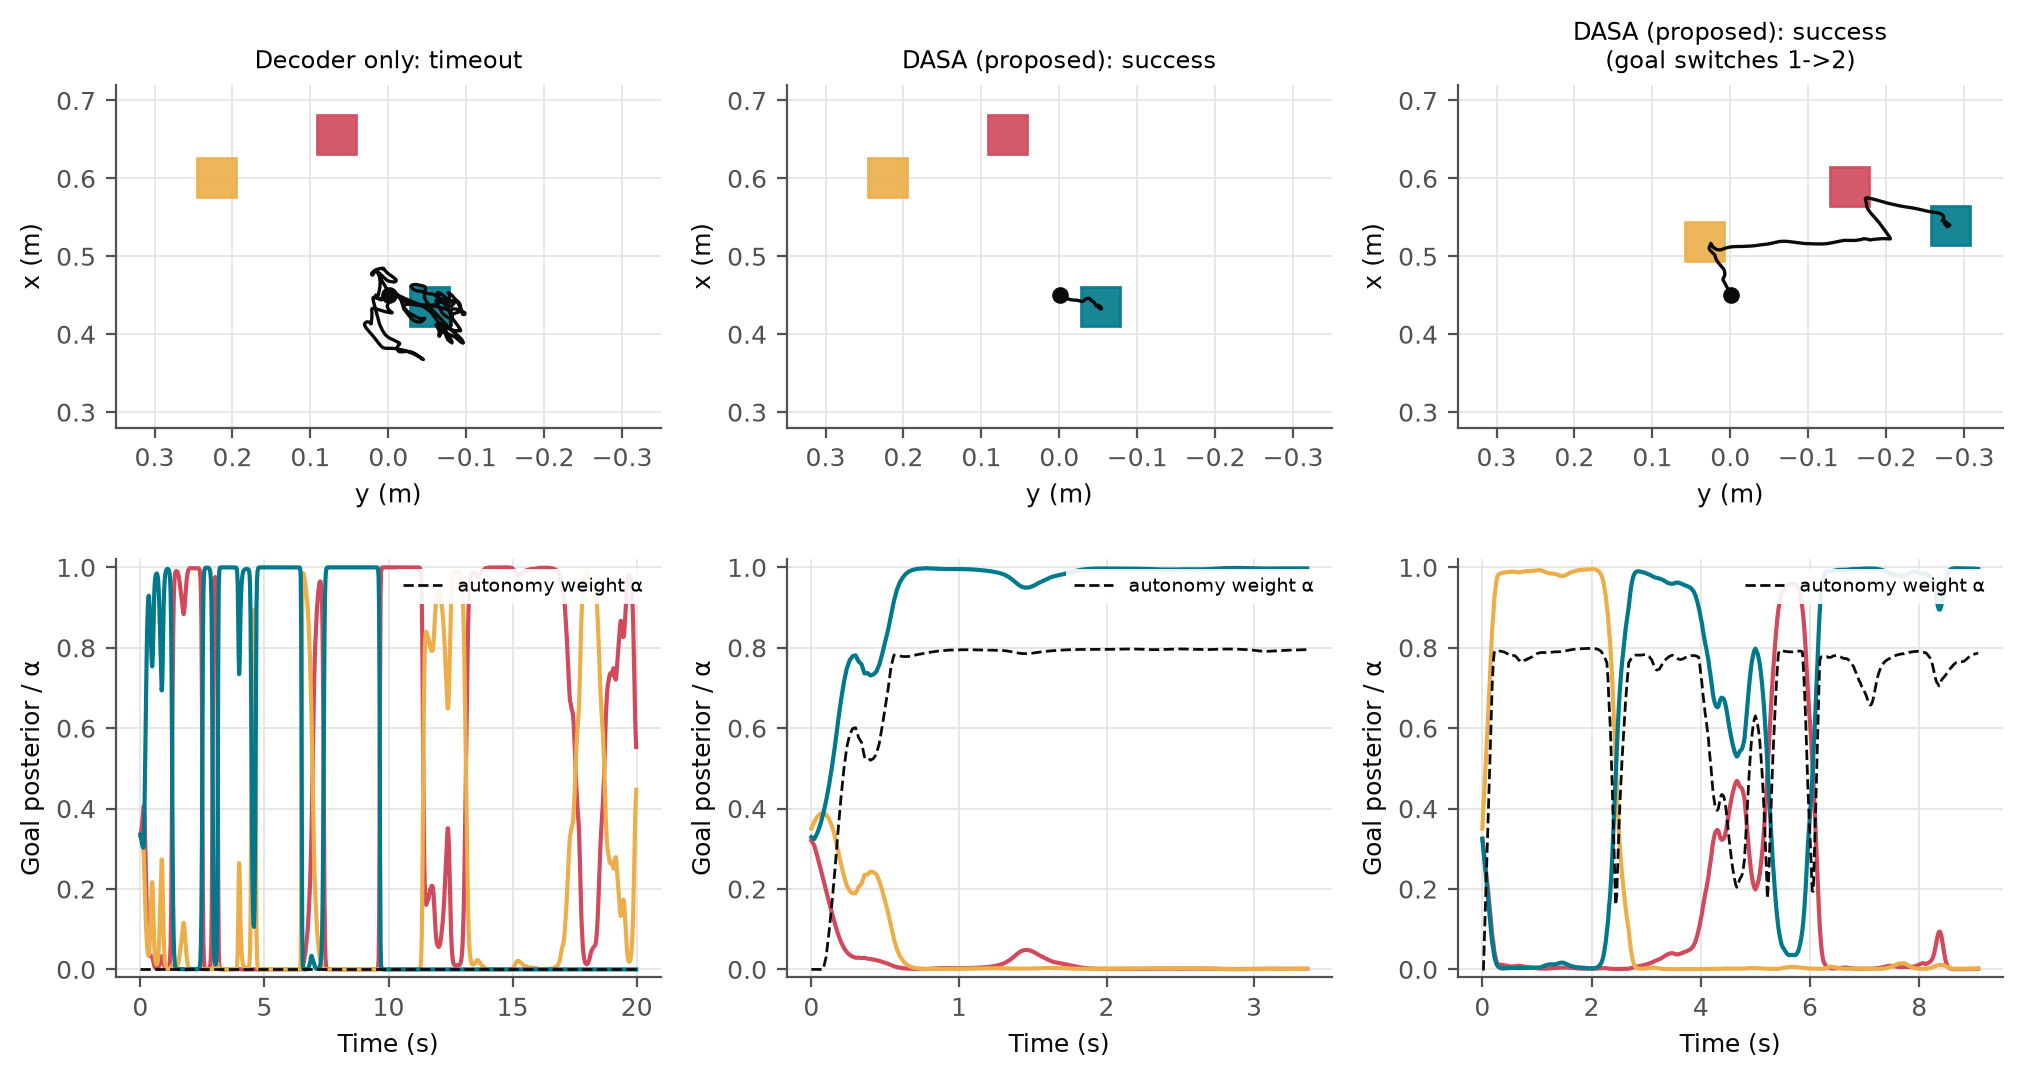
\includegraphics[width=0.78\textwidth]{figures/example_episodes.png}
\caption{Example episodes (top view; robot base at the origin, $x$ pointing away from the base). Left: decoder only on a scene where it times out. Middle: DASA on the same scene. Right: DASA with a change of mind. Bottom: goal posterior per object (object colours) and autonomy weight $\alpha$.}
\label{fig:episodes}
\end{figure*}
